% \iffalse
\let\negmedspace\undefined
\let\negthickspace\undefined
\documentclass[journal,12pt,twocolumn]{IEEEtran}
\usepackage{cite}
\usepackage{amsmath,amssymb,amsfonts,amsthm}
\usepackage{algorithmic}
\usepackage{graphicx}
\usepackage{textcomp}
\usepackage{xcolor}
\usepackage{pgfplots}
\usepackage{txfonts}
\usepackage{listings}
\usepackage{enumitem}
\usepackage{mathtools}
\usepackage{gensymb}
\usepackage{comment}
\usepackage[breaklinks=true]{hyperref}
\usepackage{tkz-euclide} 
\usepackage{listings}
\usepackage{gvv}                                        
\def\inputGnumericTable{}                                 
\usepackage[latin1]{inputenc}                                
\usepackage{color}                                            
\usepackage{array}                                            
\usepackage{longtable}                                       
\usepackage{calc}                                             
\usepackage{multirow}                                         
\usepackage{hhline}                                           
\usepackage{ifthen}                                           
\usepackage{lscape}

\newtheorem{theorem}{Theorem}[section]
\newtheorem{problem}{Problem}
\newtheorem{proposition}{Proposition}[section]
\newtheorem{lemma}{Lemma}[section]
\newtheorem{corollary}[theorem]{Corollary}
\newtheorem{example}{Example}[section]
\newtheorem{definition}[problem]{Definition}
\newcommand{\BEQA}{\begin{eqnarray}}
\newcommand{\EEQA}{\end{eqnarray}}
\newcommand{\define}{\stackrel{\triangle}{=}}
\theoremstyle{remark}
\newtheorem{rem}{Remark}
\begin{document}
\parindent 0px
\bibliographystyle{IEEEtran}
\title{GATE: EE - 7.2021}
\author{EE22BTECH11219 - Rada Sai Sujan$^{}$% <-this % stops a space
}
\maketitle
\newpage
\bigskip
\section*{Question}
Two discrete-time linear time-invarient systems with impulse responses $h_1[n]=\delta[n-1]+\delta[n+1]$ and $h_2[n]=\delta[n]+\delta[n-1]$ are connected in cascade, where $\delta[n]$ is the Kronecker delta. The impulse response of the cascaded system is   \\
\begin{enumerate}[label=(\alph*)]
    \item $\delta[n-2]+\delta[n+1]$
    \item $\delta[n-1]\delta[n]+\delta[n+1]\delta[n-1]$
    \item $\delta[n-2]+\delta[n-1]+\delta[n]+\delta[n+1]$
    \item $\delta[n]\delta[n-1]+\delta[n-2]\delta[n+1]$
\end{enumerate} \hfill(GATE 2021 EE)\\
\solution

\begin{figure}[ht]
    \centering
    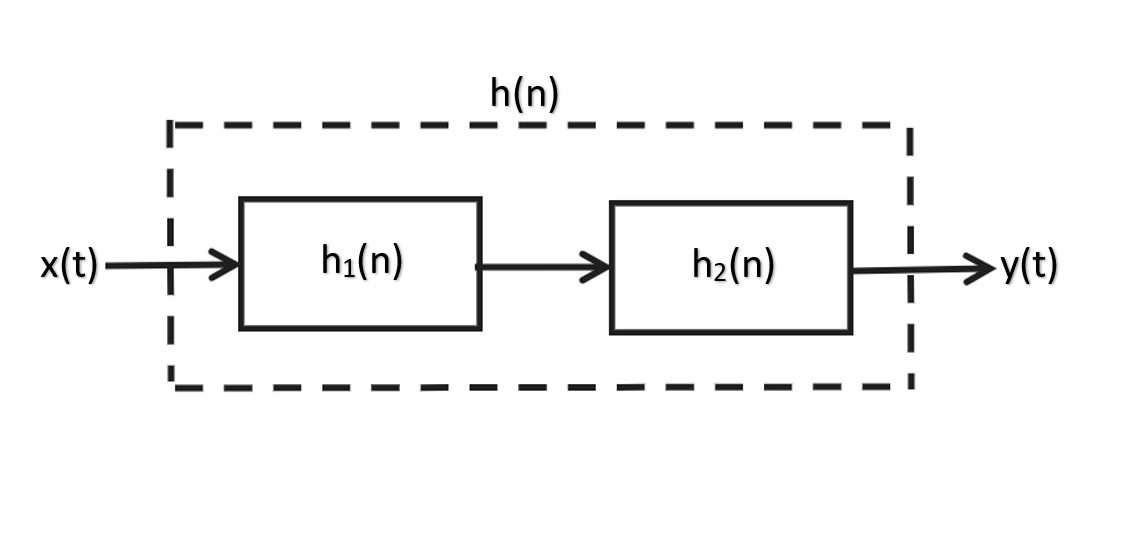
\includegraphics[width=\columnwidth]{figs/fig2.png}
    \caption{Block Diagram}
    \label{fig:g2022ee7.2}
\end{figure}  
From the $Z$-transformation pairs,
\begin{align}
    \delta[n] &\overset{\mathcal{Z}}{ \longleftrightarrow} 1  \label{eqn:g22ee7.1}  \\
    x\brak{n-k} &\overset{\mathcal{Z}}{ \longleftrightarrow} z^{-k}X\brak{z} \label{eqn:g22ee7.2}   \\
    x_1\brak{n}\ast x_2\brak{n} &\overset{\mathcal{Z}}{ \longleftrightarrow} X_1\brak{z}X_2\brak{z} \label{eqn:g22ee7.3}
\end{align}
If $h_1\brak{n}$ and $h_2\brak{n}$ are cascade connected then the resultant impulse can be given by:
\begin{align}
    h\brak{n}&=h_1\brak{n}\ast h_2\brak{n}    \\
    \implies H\brak{z}&=H_1\brak{z}H_2\brak{z}    \\
    H\brak{z}&=\brak{z^{-1}+z}\brak{1+z^{-1}}   \\
    &=\brak{z^{-1}+z^{-2}+z+1}, \quad \abs{z}\neq 0
\end{align}
Using the $Z$-transformation pairs to find the the inverse $Z$-transform,
\begin{align}
    h\brak{n}&=\delta[n-2]+\delta[n-1]+\delta[n]+\delta[n+1]
\end{align}
\begin{figure}[ht]
    \centering
    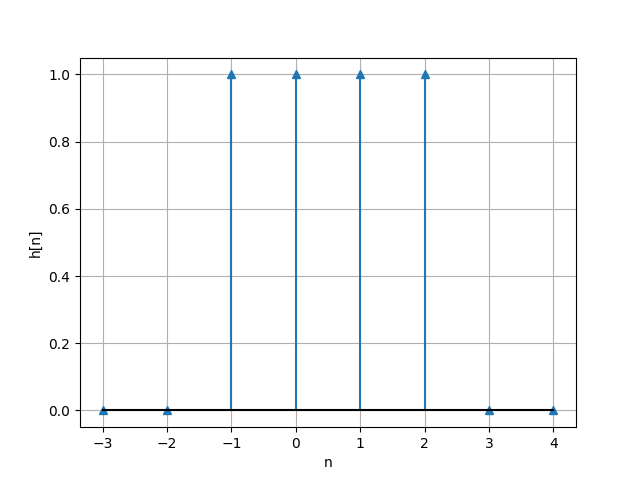
\includegraphics[width=\columnwidth]{figs/fig1.png}
    \caption{h\brak{n} $vs$ n graph}
    \label{fig:g2022ee7.1}
\end{figure}     
\end{document}
